\section{会议经费}

每位同学,无论是自费生还是奖学金学生,都有16500元的会议经费。参加会议的时候,可以用来报销注册费、住宿交通等费用。这笔钱毕业前不用完拿去\sout{在会议周边吃喝玩乐出去浪}丰富自己的学术经历就亏啦。钱虽多,申请和报销流程比较繁琐。主要资料在:
\begin{itemize}
    \item e-bridge: \url{https://ebridge.xjtlu.edu.cn/},登陆过后点击PGR Policies, Procedures and Forms,找到 \textit{Postgraduate Research Students' Conference Fund Policy} 和 \textit{
    Guideline and Procedures on Doctoral Student Travel Arrangement and Reimbursement}
    \item 官方流程图
    \begin{figure}[H]
        \centering
        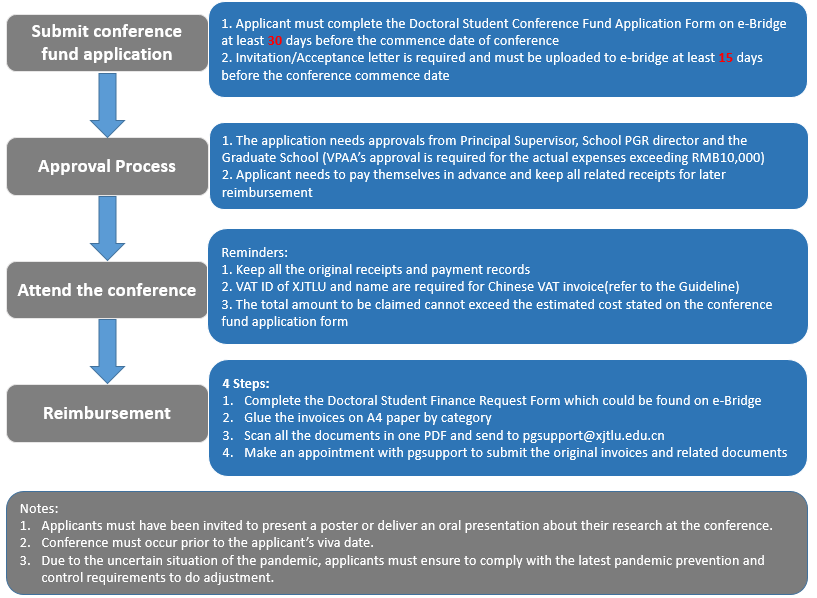
\includegraphics[width=0.9\columnwidth]{author-folder/Kai.Wu/fund-flowchart.png}
    \end{figure}
\end{itemize}

主要注意
\begin{enumerate}
    \item 必须要至少提前30天申请。因此不能用于“你突然听说有个30天内要开的会议”
    \item 必须要在会议上作报告,poster或者oral都可以,否则不能使用经费
    \item 不能使用学校经费的时候,可能可以使用你导师的某些经费。我就因为上述原因,用导师的经费报销过几场会议。具体怎么做\&你导师到底有没有这种经费,问你自己的导师
\end{enumerate}


\begin{flushright}
(2022年10月12日 by Kai Wu)
\end{flushright}